\chapter{Architecture}
\label{cap:method}

This chapter presents the proposed solution and describes the architecture and its components. The architecture is designed to be scalable and cloud-agnostic, capable of collecting, processing, and storing IoT data flexibly and resiliently meaning that the architecture’s is able to recover from failures or disruptions while maintaining its core functions.



\begin{figure}[htbp]
    \centering
    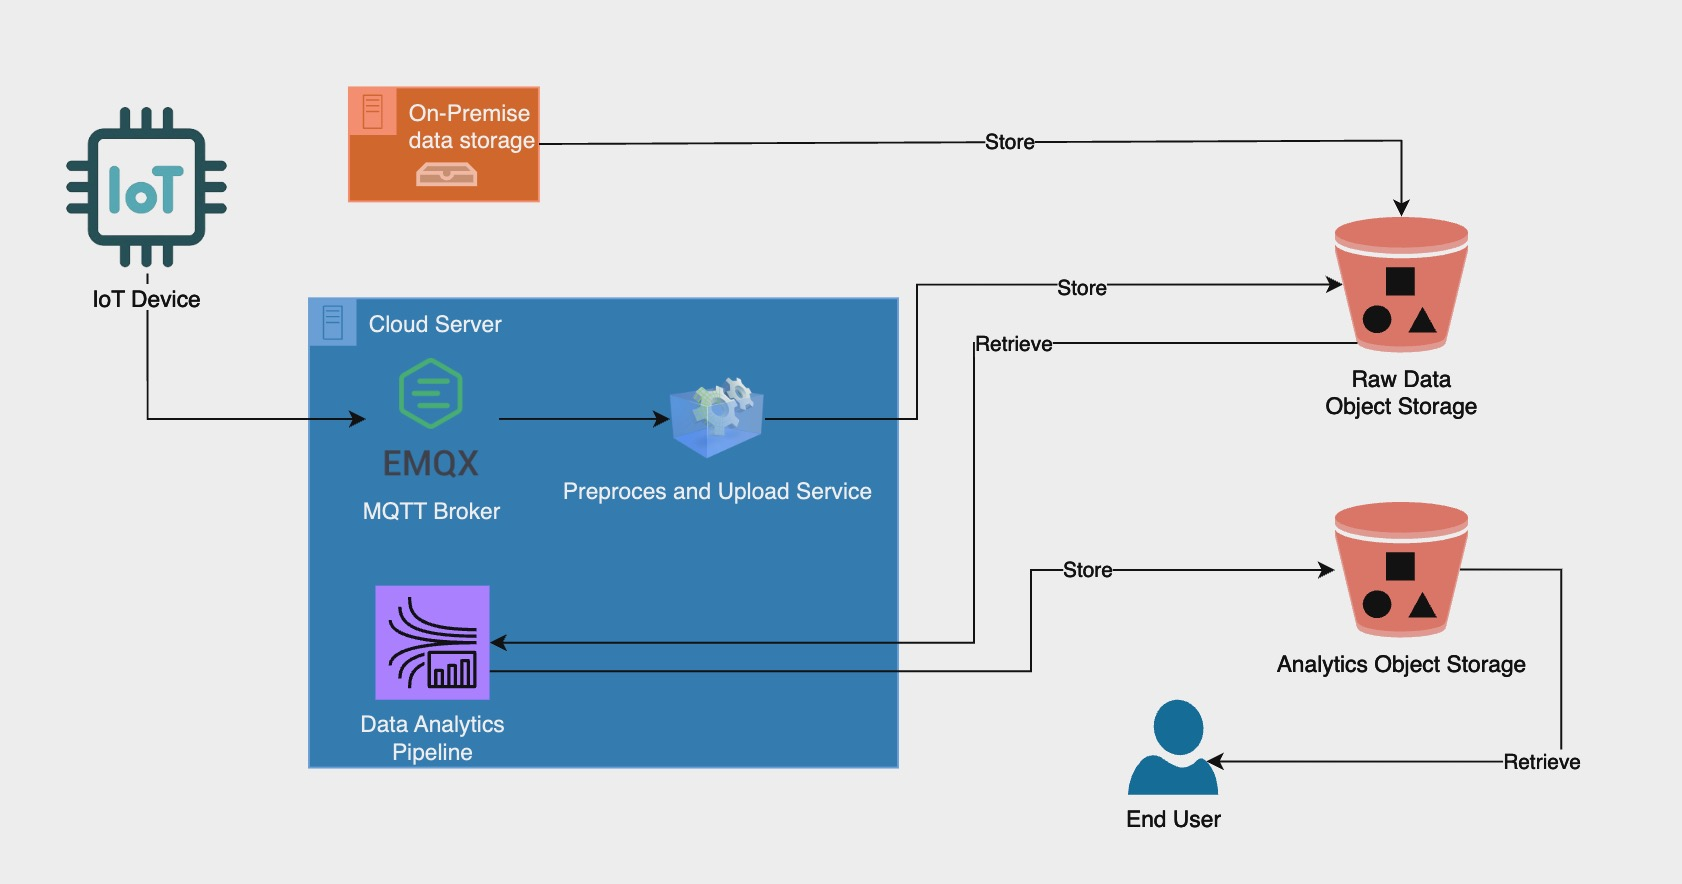
\includegraphics[width=1\textwidth]{Immagini/architecture.png}
    \caption{Architecture of the proposed solution}
    \label{fig:architecture}
\end{figure}

The architecture shown in figure \ref{fig:architecture} is based on a modular, microservices approach. It is divided into three key layers: the data collection layer, the data storage layer, and the data analysis layer. Each layer addresses specific aspects of IoT data management, ensuring scalability, flexibility, and cloud-agnostic capabilities. The architecture is designed to handle large volumes of data from IoT devices and archive data sources.

\section{Data collection layer}

The data collection layer is responsible for ingesting data from various IoT devices and data which is already archived on on-premise systems. This layer must support real-time data ingestion from IoT devices, as well as batch uploads of historical data.

\subsection{Data collection from IoT devices}
IoT devices send data to a cloud-hosted MQTT broker using the MQTT protocol, which is suitable for environments with limited bandwidth. Each IoT device publishes its data under specific MQTT topics, allowing for organized and efficient data routing. The collected data is structured in JSON format and contains timestamps and sensor readings. Before storage, the data is converted to CSV format for easier processing and analysis.

\subsection{Data collection from archived data}
The system also handles historical data uploads from on-premise sources. A simple script is used to upload archived CSV files to the cloud via the cloud provider's API. The data does not require preprocessing and is stored directly in object storage, making it available for further analysis.

\section{Data storage layer}

The data storage layer is designed to store both raw and analyzed data, using object storage as the primary storage solution. Object storage offers scalability, durability, and global accessibility, which makes it ideal for IoT data management. The architecture separates the storage of raw data from analyzed data by using different storage buckets, simplifying data management and ensuring efficient access to data for analysis.

This storage layer is inherently cloud-agnostic, as all major cloud providers offer similar object storage services. The solution can be deployed on any cloud provider with minimal adjustments, ensuring flexibility and avoiding vendor lock-in.

\section{Data analysis layer}

The data analysis layer retrieves preprocessed data from object storage for further processing and analysis. This layer supports a range of analytics operations, from simple statistical analysis to advanced machine learning and deep learning models. Data is first downloaded from the object storage to a local compute instance, as direct access to object storage file contents is not supported by cloud platforms.

Once the data is processed, the results are uploaded back to object storage in a separate bucket for easy access by other services or users. Data analysis can be triggered either automatically when new data is uploaded or by the user via an API call, depending on the specific requirements of the system.

\section{Cloud server (IaaS) vs. SaaS solutions}

The architecture makes use of Infrastructure as a Service (IaaS) to host the MQTT broker and the data analytics pipeline. While Software as a Service (SaaS) solutions offer convenience, the flexibility provided by IaaS allows for more control over the infrastructure and supports custom configurations and library dependencies needed for the data analytics pipeline.

This approach also ensures that the system remains cloud-agnostic. Since all major cloud providers offer IaaS services, the architecture can be deployed on any platform without requiring significant modifications. Additionally, using IaaS gives the system better cost control over time, as pricing can be optimized based on the specific needs of the workload.

\section{Why the Proposed Architecture is Scalable}

Scalability is a core feature of the proposed architecture, allowing it to handle increasing volumes of data and expanding workloads without significant changes to the underlying structure. The system achieves scalability through several design principles:

\begin{itemize}
    \item \textbf{Microservices Architecture}: The architecture follows a microservices-based design, where different components (such as data collection, storage, and analysis) are loosely coupled and operate independently. This allows each service to be scaled independently based on the workload it handles. For example, the data analysis service can be scaled up to handle more intensive computations, while the data storage service can be scaled based on the amount of incoming data.
    
    \item \textbf{Horizontal and Vertical Scaling}: The architecture supports both horizontal scaling (adding more servers or instances to distribute the load) and vertical scaling (increasing the resources of existing servers). In the case of IoT data, which can grow a lot when lots of devices are connected, horizontal scaling is particularly valuable. For instance, additional computing servers can be added as the number of connected IoT devices increases. 
    
    \item \textbf{Cloud Infrastructure}: By utilizing cloud services such as Infrastructure as a Service (IaaS) and Object Storage, the architecture can leverage the inherent scalability of cloud platforms. Cloud providers offer auto-scaling features, enabling the system to automatically adjust resource allocation based on demand. This ensures that the architecture can handle variable workloads without manual intervention.

    \item \textbf{Object Storage}: The use of object storage allows the system to scale storage capacity without the need for complex infrastructure changes. Object storage systems are designed to handle vast amounts of unstructured data, making them ideal for IoT environments where data volume can increase rapidly. Since object storage scales automatically with the amount of data, the system can store large volumes of raw and processed data without performance degradation.
    
    \item \textbf{Distributed Data Processing}: The data analysis layer supports distributed data processing, allowing the workload to be spread across multiple servers or instances. This makes it possible to handle large-scale analytics tasks efficiently. Distributed processing frameworks such as Apache Spark could be integrated to perform parallel processing of large datasets, enhancing the system’s capacity to handle intensive computational tasks.

    \item \textbf{Event-Driven Architecture}: The system's event-driven design, particularly in the data collection and analysis layers, enables automatic scaling based on real-time data flow. When new data arrives, events can trigger scaling actions, such as adding more compute resources for analysis, ensuring that the system remains responsive even under high demand.
\end{itemize}

Overall, the architecture’s design ensures that it can scale in response to both growing data volumes and increased computational demands, making it suitable for a wide range of IoT applications. This scalability, combined with its cloud-agnostic nature, ensures that the system can grow and adapt without significant redesigns or performance trade-offs.


\section{Why the proposed architecture is cloud-agnostic}

The proposed architecture is designed to operate seamlessly on any cloud platform by leveraging standardized services and protocols. Key elements that make this architecture cloud-agnostic include:

\begin{itemize}
    \item \textbf{Object Storage}: The data storage layer uses object storage for both raw and processed data. Object storage services are available across all major cloud platforms, ensuring seamless integration with any provider.
    \item \textbf{MQTT Protocol}: The data collection layer uses MQTT, a lightweight messaging protocol widely supported by different cloud providers. This ensures flexibility and compatibility with various cloud-hosted or self-hosted MQTT brokers.
    \item \textbf{IaaS Services}: The use of IaaS to host the broker and data analysis services makes the system platform-independent. Any cloud provider that supports IaaS can host the solution without changes to the architecture.
\end{itemize}

By designing the system to use standardized components and protocols, the architecture ensures that the solution can be deployed on any cloud provider, reducing the risk of vendor lock-in and enhancing the ability to scale and adapt to different environments.
